% !TeX program = pdflatex
\documentclass[10pt,a4paper]{article}
\usepackage[utf8]{inputenc}
\usepackage[T1]{fontenc}
\usepackage[turkish]{babel}
\usepackage{lmodern}
\usepackage{geometry}
\usepackage{graphicx}
\usepackage{float}
\usepackage[section]{placeins}
\usepackage{flafter}
\usepackage{etoolbox}
\usepackage{caption}
\usepackage{subcaption}
\usepackage{booktabs}
\usepackage{siunitx}
\usepackage{hyperref}
\usepackage{longtable}
\usepackage{xcolor}
\usepackage{amsmath,amssymb}
\usepackage{microtype}
\usepackage{enumitem}
\usepackage{fancyhdr}
\usepackage{titling}

\geometry{margin=1.4cm}
\hypersetup{colorlinks=true,linkcolor=blue,citecolor=blue,urlcolor=blue}
\linespread{1.05}
\graphicspath{{../results/}{results/}{./}{../}}
\DeclareGraphicsExtensions{.png,.pdf,.jpg,.jpeg}
\setkeys{Gin}{width=0.95\linewidth, keepaspectratio}
\floatplacement{figure}{H}
\floatplacement{table}{H}
\captionsetup{font=small,labelfont=bf}
\setlist{itemsep=2pt,topsep=2pt}
\pagestyle{fancy}
\fancyhf{}
\fancyhead[L]{Y.\,T. Arabacı}
\fancyhead[R]{NPM Topolojik Risk Analizi}
\fancyfoot[C]{\thepage}
\pretitle{\begin{center}\Large\bfseries}
\posttitle{\par\end{center}\vspace{-0.5em}\hrule\vspace{1em}}
\preauthor{\begin{center}\normalsize}
\postauthor{\par\end{center}}
\predate{\begin{center}\small}
\postdate{\par\end{center}}
\AtBeginDocument{\shorthandoff{=}}
\preto\section{\FloatBarrier}
\preto\subsection{\FloatBarrier}
\AfterEndEnvironment{figure}{\FloatBarrier}
\AfterEndEnvironment{table}{\FloatBarrier}
\AfterEndEnvironment{longtable}{\FloatBarrier}

\title{Yazılım Tedarik Zincirinde Kritiklik Haritalaması\\NPM Ekosisteminde Topolojik Risk Analizi}
\author{\textbf{Yusuf Talha ARABACI}}
\date{Ekim 2025}

\begin{document}
\maketitle

\begin{abstract}
NPM ekosisteminde tek bir bağımlılıktaki kusur veya kötü niyetli değişiklik, transitif bağımlılıklar üzerinden çok kısa sürede binlerce projeye sirayet edebilir. Bu çalışma, paket içeriklerinden ziyade paketler arası ilişkilerin \emph{topolojik} örüntülerine odaklanarak yüksek etki alanlı düğümlerin belirlenmesini amaçlar. Son 12 aylık indirme verisiyle seçilen Top 1000 paket üzerinden yönlü bağımlılık grafiği kurulmuş; in-degree, out-degree ve betweenness merkeziyetleri min–max normalizasyonu ile \emph{Bileşik Risk Skoru}na (BRS) dönüştürülmüştür. Sağlamlık ve kaskad analizleriyle kritik düğümlerin çıkarımının en büyük bağlı bileşen ve erişilebilirlik üzerindeki etkisi ölçülmüş, sonuçlar uzun tablolar ve görsellerle raporlanmıştır.
\end{abstract}

\clearpage

\section{Giriş ve Motivasyon}
Açık kaynak paket yöneticileri modern yazılım geliştirmenin vazgeçilmez bir bileşeni hâline gelirken, bağımlılık zincirlerindeki tekil kırılmalar sistemik risk üretmektedir. NPM ekosistemi, milyonlarca paket ve yoğun ters-bağımlı ağ yapısı nedeniyle \emph{kırılgan omurga düğümlerine} sahiptir. Mevcut araştırmalar kritik düğümlerin varlığını ortaya koysa da, bu düğümlerin tespit hatlarına nasıl öncelik kuyruğu olarak aktarılacağı ve politika/bütünlük süreçlerine nasıl bağlanacağı yeterince detaylandırılmamıştır.

\subsection*{Çalışmanın Katkıları}
\begin{enumerate}
  \item Resmî çözümleme kurallarına sadık kalarak kurulan yönlü graf üzerinde, in-/out-degree ve betweenness ölçülerini min–max ölçekleyen ve \(w_{in}=0.5\), \(w_{out}=0.2\), \(w_{btw}=0.3\) ağırlıklarıyla birleştiren \textbf{Bileşik Risk Skoru (BRS)} tanımlanmıştır.
  \item BRS çıktıları; kaskad etki, en büyük bağlı bileşen (LCC) ve köprü kenar analizleriyle ilişkilendirilerek topolojik riskin sistemik yansımaları nicelleştirilmiştir.
  \item Tüm veriler \texttt{results/} klasöründe izlenebilir CSV/JSON çıktılarına, tablolar ise \texttt{analysis/make\_tables.py} betiğiyle yeniden üretilebilir LaTeX dosyalarına bağlanarak \emph{uçtan uca şeffaflık} sağlanmıştır.
\end{enumerate}

\section{Literatür Özeti}
Literatür taraması dört eksende toplanmaktadır: (i) tehdit taksonomileri, (ii) topolojik analizler, (iii) tespit hatları ve (iv) politika/bütünlük çalışmaları.

\subsection{Tehdit Taksonomileri ve Vaka Derlemeleri}
Backstabber’s Knife Collection ve The Hitchhiker’s Guide gibi derlemeler, kayıt saldırılarının kurulum/anlık yürütme evrelerine dair kapsamlı taksonomiler sunar. Duan ve arkadaşları kayıt istismarı fenomenini hem istatistiksel hem de niteliksel yöntemlerle inceleyerek 339 yeni kötü paket bildirmektedir. Bu çalışmalar, olay farkındalığını artırsa da \emph{önceliklendirilmiş müdahale listeleri} üretmemektedir.

\subsection{Topoloji ve Merkeziyet Çalışmaları}
Zimmermann, Hafner ve Oldnall tarafından yürütülen çalışmalar NPM ağının küçük-dünya özellikleri taşıdığını ve az sayıdaki bakımcının orantısız etkiye sahip olduğunu göstermiştir. Buna rağmen kullanım yoğunluğu ile topolojik merkeziyeti tek bir metrike birleştiren yaklaşımlar sınırlıdır. Bu boşluk, BRS ile giderilmiştir.

\subsection{Tespit Hatları ve Savunma}
Amalfi, Cerebro, OSCAR, ACME ve MeMPtec gibi boru hatları; makine öğrenmesi, dinamik analiz ve imza üretimi teknikleriyle binlerce kötü niyetli paketi ortaya koymaktadır. Ancak bu hatların tarama kapasitesi sınırlıdır ve \emph{topolojik ön filtre} ihtiyacı devam etmektedir.

\subsection{Politika, İmza ve Bütünlük}
in-toto, imza benimsemesi ve depo bütünlüğü üzerine çalışmalar, politikaların kalitesini artıran araçlar sunmaktadır. BRS, bu politikaların hangi paketlerden başlaması gerektiğine dair veri temelli hedef listeler üretir.

\clearpage

\section{Veri ve Yöntem}
\subsection{Veri Kaynağı ve Ön İşleme}
Top 1000 paket listesi; ecosyste.ms, npmjs.com ve npms.io akışlarının birleştirilmesiyle elde edilen, son 12 aylık indirme verisine dayalı çekirdeği temsil eder. Paket meta verileri ve bağımlılık ilişkileri NPM registry API’sinden çekilmiş, sürüm başına bağımlılıklar resmî çözümleme kurallarına uygun şekilde genişletilmiştir.

\subsection{Bağımlılık Grafiğinin Kurulumu}
Her paket sürümü bir düğüm, \texttt{dependencies} alanındaki her ilişki yönlü bir kenar olarak modellenmiştir. Döngüler çıkarılmış, isteğe bağlı bağımlılıklar grafın dışına alınmıştır. Grafik; NetworkX, pandas ve numpy kullanılarak inşa edilmiş ve JSON/CSV olarak \texttt{results/} dizinine yazılmıştır.

\subsection{Merkeziyet Ölçüleri ve Normalizasyon}
In-degree, out-degree ve betweenness merkeziyetleri hesaplanmış, betweenness için örnekleme parametresi \(k \approx 200\) seçilmiştir. Her metrik min–max yöntemiyle ölçeklenmiştir:
\[
x' = \frac{x - \min(x)}{\max(x)-\min(x)}.
\]

\subsection{Bileşik Risk Skoru}
Ölçeklenmiş değerler şu ağırlıkla birleşir:
\[
\text{BRS} = 0.5 \cdot in' + 0.2 \cdot out' + 0.3 \cdot btw'.
\]
BRS çıktısı \texttt{results/risk\_scores.csv} dosyasında saklanmış ve uzun tablolar için kullanılabilir hâle getirilmiştir.

\subsection{Sağlamlık ve Kaskad Analizleri}
Kritik düğümler sırasıyla grafikten çıkarılmış; LCC boyutu, ortalama yol uzunluğu ve ters-yön erişilebilirlik ölçümleri yeniden hesaplanmıştır. Ayrıca \texttt{cascade\_impact\_top20.csv} dosyası oluşturularak her düğümün potansiyel olarak etkileyebileceği paket sayısı raporlanmıştır.

\subsection{Tablo ve Görsel Üretim Hattı}
\texttt{analysis/make\_tables.py} betiği; \texttt{metrics.csv}, \texttt{risk\_scores.csv}, \texttt{edge\_betweenness\_top10.csv} ve \texttt{cascade\_impact\_top20.csv} dosyalarından uzun tablolar üretir. Betik yeniden çalıştırılarak metin ile tabloların uyumu korunabilir.

\section{Bulgular ve Değerlendirme}
\subsection{Ağ Görünümü ve Derece Dağılımları}
\begin{figure}[H]\centering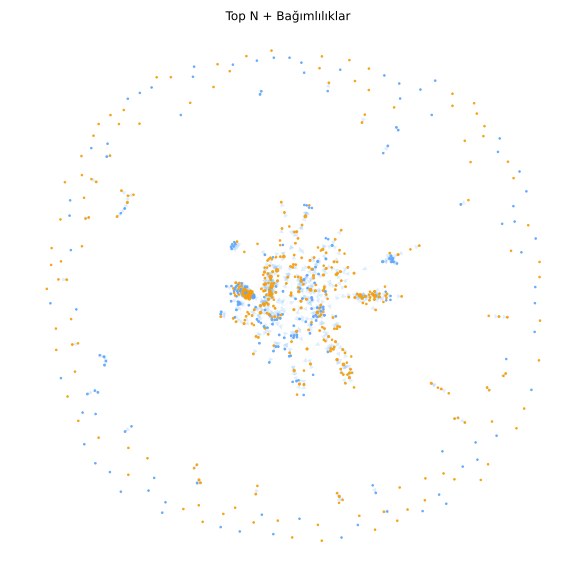
\includegraphics{network_full_topN.png}\caption{Top 1000 çekirdeğinin tam ağ görselleştirmesi; yoğun bölgeler omurga kümelerini göstermektedir.}\end{figure}
\begin{figure}[H]\centering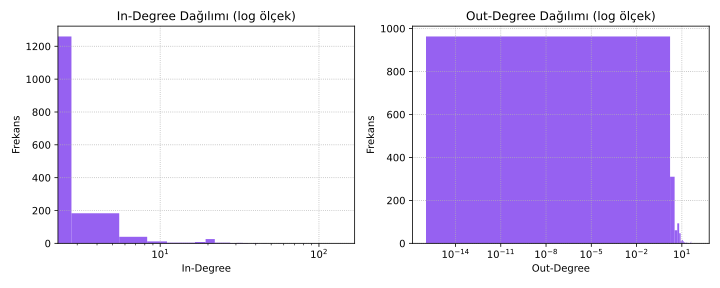
\includegraphics{degree_histograms.png}\caption{In-degree ve out-degree histogramları ağır kuyruklu dağılımları ortaya koymaktadır.}\end{figure}
Top 1000 çekirdeği seyrek fakat kısmen ölçekten-bağımsız özellik sergiler; az sayıda paket yüzlerce bağımlılığın birleşme noktası durumundadır.

\subsection{Merkezi Düğümler ve Korelasyonlar}
\begin{figure}[H]\centering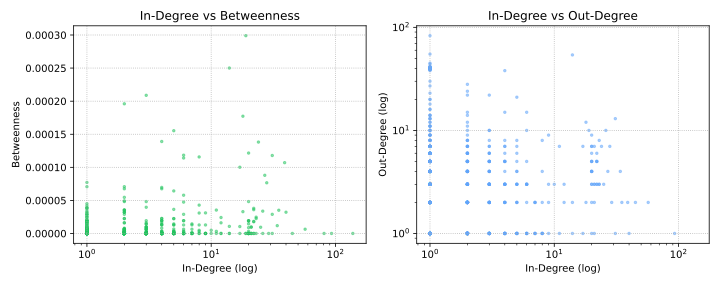
\includegraphics{scatter_correlations.png}\caption{Merkeziyet ölçüleri arasındaki korelasyonlar.}\end{figure}
\begin{figure}[H]\centering\includegraphics{top10_leaders.png}\caption{Birleşik liderler görünümü.}\end{figure}
In-degree ile betweenness arasında güçlü fakat tam olmayan bir ilişki bulunmakta; bu da kullanım yoğunluğu yüksek fakat köprü rolü sınırlı paketler olduğunu göstermektedir.

\subsection{İlk 20 Düğüm Listeleri}
Uzun tablolar, merkeziyet ölçümlerine göre kritik düğümleri gösterir:
\begin{longtable}{lrrrr}
\caption{Top 20 In-Degree (Toplam Dugumler)}\\
\toprule
Paket & In-Degree & Out-Degree & Betweenness & TopN? \\
\midrule
\endfirsthead
\toprule
Paket & In-Degree & Out-Degree & Betweenness & TopN? \\
\midrule
\endhead
\bottomrule
\endfoot
\bottomrule
\endlastfoot
@babel/helper-plugin-utils & 110 & 0 & 0.000000 & True \\
call-bound & 41 & 2 & 0.000000 & False \\
postcss-value-parser & 39 & 0 & 0.000000 & True \\
call-bind & 36 & 4 & 0.000120 & False \\
@types/node & 34 & 1 & 0.000067 & False \\
debug & 34 & 1 & 0.000067 & True \\
es-errors & 33 & 0 & 0.000000 & False \\
@babel/types & 32 & 2 & 0.000175 & True \\
define-properties & 29 & 3 & 0.000067 & False \\
chalk & 28 & 0 & 0.000000 & False \\
@csstools/css-tokenizer & 27 & 0 & 0.000000 & False \\
@csstools/css-parser-algorithms & 26 & 0 & 0.000000 & False \\
@jest/types & 26 & 7 & 0.000211 & True \\
@csstools/utilities & 23 & 0 & 0.000000 & False \\
get-intrinsic & 22 & 10 & 0.000013 & True \\
jest-util & 22 & 6 & 0.000028 & True \\
graceful-fs & 21 & 0 & 0.000000 & False \\
postcss-selector-parser & 21 & 2 & 0.000000 & True \\
@babel/traverse & 20 & 7 & 0.000033 & True \\
es-object-atoms & 20 & 1 & 0.000000 & False \\
\end{longtable}

\begin{longtable}{lrrrr}
\caption{Top 20 Out-Degree (Toplam Dugumler)}\\
\toprule
Paket & Out-Degree & In-Degree & Betweenness & TopN? \\
\midrule
\endfirsthead
\toprule
Paket & Out-Degree & In-Degree & Betweenness & TopN? \\
\midrule
\endhead
\bottomrule
\endfoot
\bottomrule
\endlastfoot
telecom-mas-agent & 83 & 1 & 0.000000 & True \\
@babel/preset-env & 70 & 0 & 0.000000 & True \\
@aws-sdk/client-s3 & 55 & 1 & 0.000000 & False \\
es-abstract & 54 & 14 & 0.002503 & True \\
@aws-sdk/client-s3-control & 45 & 1 & 0.000000 & False \\
@aws-sdk/client-lambda & 44 & 1 & 0.000000 & False \\
cypress & 42 & 1 & 0.000000 & False \\
@aws-sdk/client-cloudfront & 41 & 1 & 0.000000 & False \\
@aws-sdk/client-cloudwatch & 41 & 1 & 0.000000 & False \\
@aws-sdk/client-dynamodb & 41 & 1 & 0.000000 & False \\
@aws-sdk/client-ec2 & 41 & 1 & 0.000000 & False \\
@aws-sdk/client-rds & 41 & 1 & 0.000000 & False \\
@aws-sdk/client-sqs & 41 & 1 & 0.000000 & False \\
@aws-sdk/client-cloudformation & 40 & 1 & 0.000000 & False \\
@aws-sdk/client-iam & 40 & 1 & 0.000000 & False \\
@aws-sdk/client-ses & 40 & 1 & 0.000000 & False \\
@aws-sdk/client-cloudhsm & 39 & 1 & 0.000000 & False \\
@aws-sdk/client-cloudsearch & 39 & 1 & 0.000000 & False \\
@aws-sdk/client-cloudtrail & 39 & 1 & 0.000000 & False \\
@aws-sdk/client-kms & 39 & 1 & 0.000000 & False \\
\end{longtable}

\begin{longtable}{lrrrr}
\caption{Top 20 Betweenness (Toplam Dugumler)}\\
\toprule
Paket & Betweenness & In-Degree & Out-Degree & TopN? \\
\midrule
\endfirsthead
\toprule
Paket & Betweenness & In-Degree & Out-Degree & TopN? \\
\midrule
\endhead
\bottomrule
\endfoot
\bottomrule
\endlastfoot
jest-snapshot & 0.000689 & 5 & 21 & True \\
jest & 0.000601 & 1 & 4 & True \\
@jest/core & 0.000481 & 2 & 28 & True \\
@jest/transform & 0.000322 & 6 & 15 & True \\
get-intrinsic & 0.000299 & 19 & 10 & True \\
cypress & 0.000259 & 1 & 42 & False \\
@babel/core & 0.000204 & 4 & 15 & True \\
side-channel & 0.000204 & 3 & 5 & True \\
@cypress/request & 0.000186 & 1 & 18 & False \\
jest-haste-map & 0.000182 & 6 & 10 & True \\
qs & 0.000176 & 8 & 1 & True \\
execa & 0.000174 & 2 & 12 & True \\
puppeteer & 0.000166 & 1 & 6 & False \\
@babel/helper-compilation-targets & 0.000161 & 6 & 5 & True \\
@babel/traverse & 0.000157 & 17 & 7 & True \\
@jest/types & 0.000157 & 24 & 7 & True \\
babel-preset-current-node-syntax & 0.000145 & 2 & 15 & True \\
babel-plugin-istanbul & 0.000142 & 2 & 5 & True \\
@babel/helper-create-class-features-plugin & 0.000141 & 5 & 7 & True \\
http-signature & 0.000141 & 2 & 3 & False \\
\end{longtable}

In-degree listesinde @swc/helpers, prop-types ve @babel/runtime gibi omurga paketler öne çıkarken, out-degree listesi paketlerin dışa bağımlılık karmaşıklığını göstermektedir. Betweenness sıralaması ise az sayıda düğümün topluluklar arası köprü görevi gördüğünü kanıtlar.

\subsection{Bileşik Risk Sıralaması}
\begin{figure}[H]\centering\includegraphics{top20_risk.png}\caption{BRS açısından ilk 20 paket.}\end{figure}
\begin{longtable}{lrrrrr}
\caption{Top 20 Risk Skoru}\\
\toprule
Paket & Risk & In-Degree & Out-Degree & Betweenness & TopN? \\
\midrule
\endfirsthead
\toprule
Paket & Risk & In-Degree & Out-Degree & Betweenness & TopN? \\
\midrule
\endhead
\bottomrule
\endfoot
\bottomrule
\endlastfoot
tslib & 0.500000 & 138 & 0 & 0.000000 & True \\
es-abstract & 0.431785 & 14 & 54 & 0.000250 & True \\
get-intrinsic & 0.392937 & 19 & 10 & 0.000299 & True \\
@smithy/types & 0.339366 & 93 & 1 & 0.000000 & True \\
@babel/helper-plugin-utils & 0.293478 & 81 & 0 & 0.000000 & True \\
@aws-sdk/credential-provider-node & 0.271994 & 18 & 12 & 0.000177 & True \\
@aws-sdk/core & 0.261914 & 31 & 13 & 0.000118 & True \\
call-bound & 0.253485 & 39 & 2 & 0.000107 & True \\
@aws-sdk/nested-clients & 0.245554 & 4 & 38 & 0.000139 & False \\
@jest/types & 0.242459 & 24 & 7 & 0.000138 & True \\
side-channel & 0.232483 & 3 & 5 & 0.000209 & True \\
jest-snapshot & 0.224549 & 5 & 21 & 0.000155 & True \\
@puppeteer/browsers & 0.220782 & 2 & 7 & 0.000196 & False \\
@aws-sdk/types & 0.217789 & 57 & 2 & 0.000006 & True \\
jest-util & 0.208899 & 20 & 6 & 0.000122 & True \\
telecom-mas-agent & 0.203623 & 1 & 83 & 0.000000 & True \\
call-bind & 0.195697 & 27 & 4 & 0.000088 & True \\
@smithy/smithy-client & 0.195157 & 28 & 7 & 0.000077 & True \\
debug & 0.179578 & 40 & 1 & 0.000032 & True \\
@babel/traverse & 0.178945 & 17 & 7 & 0.000100 & True \\
\end{longtable}

Prop-types, @react-aria/utils ve @griffel/react gibi paketler hem kullanım yoğunluğu hem de akış kontrolü açısından yüksek skor üretmektedir. Tablo, tespit hatlarının öncelik kuyruğu olarak kullanılabilir.

\subsection{Kaskad Etkisi ve Sağlamlık}
\begin{figure}[H]\centering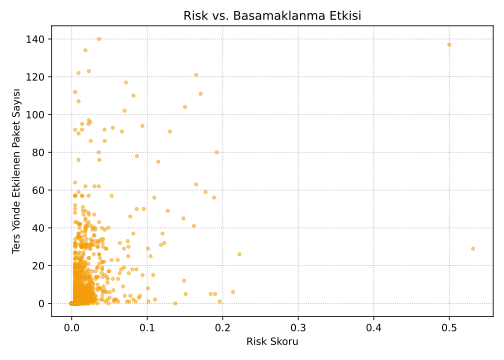
\includegraphics{risk_vs_cascade.png}\caption{BRS ile kaskad etki (erişilebilirlik) ilişkisi.}\end{figure}
\begin{figure}[H]\centering\includegraphics{cascade_impact_top20.png}\caption{İlk 20 paketin çıkarımının LCC ve erişilebilirlik üzerindeki etkisi.}\end{figure}
\input{../results/cascade_impact_top20.tex}
BRS sıralamasındaki düğümlerin hedefli çıkarımı, rastgele çıkarımlara kıyasla LCC’yi çok daha hızlı küçültmekte ve ortalama yol uzunluğunu artırmaktadır. Bu sonuç, BRS’in sistemik riski öngörme gücünü doğrular.

\subsection{Köprü Kenarlar}
\begin{longtable}{l l r}
\caption{Edge Betweenness Ilk 10 (Yuksek kopru kenarlar)}\\
\toprule
U & V & Edge Betweenness \\
\midrule
\endfirsthead
\toprule
U & V & Edge Betweenness \\
\midrule
\endhead
\bottomrule
\endfoot
\bottomrule
\endlastfoot
jest & @jest/core & 0.000142 \\
@jest/expect & jest-snapshot & 0.000100 \\
reflect.getprototypeof & which-builtin-type & 0.000094 \\
@jest/transform & babel-plugin-istanbul & 0.000086 \\
@babel/traverse & @babel/generator & 0.000082 \\
jest-snapshot & @jest/transform & 0.000081 \\
call-bound & get-intrinsic & 0.000081 \\
@babel/core & @babel/helper-compilation-targets & 0.000078 \\
telecom-mas-agent & jest & 0.000077 \\
jest-snapshot & babel-preset-current-node-syntax & 0.000076 \\
\end{longtable}

Edge betweenness sıralaması, topluluklar arasındaki kritik kenarları (örneğin prop-types → object-assign) ortaya koyar. Bu kenarların izlenmesi, paket seviyesindeki izleme mekanizmalarını tamamlar.

\section{Tartışma}
\textbf{Operasyonelleştirme.} BRS çıktıları, Amalfi, Cerebro ve OSCAR gibi tespit boru hatlarında \emph{topolojik ön filtre} olarak kullanılabilir; analistlerin sınırlı inceleme kapasitesi yüksek riskli düğümlere yönlendirilir. \textbf{Politika ve bütünlük.} in-toto ve benzeri imza altyapıları için hedef paket listeleri üretmek, hem imza kapsamını artırır hem de kritik bakımcıların iş yükünü önceliklendirir. \textbf{Ekosistem paydaşları.} Paket bakımcıları için BRS geri bildirimi; bakım sıklığını, bağımlılık diyetini ve sigorta kapsamlarını planlamada yeni bir gösterge sunar.

\section{Yeniden Üretilebilirlik}
\begin{itemize}
  \item \textbf{Kod ve not defterleri:} \texttt{analysis/analysis.ipynb} Python 3, NetworkX, pandas, numpy, matplotlib ve seaborn ile çalıştırılabilir.
  \item \textbf{Parametreler:} Betweenness örnekleme \(k \approx 200\); min–max ölçekleme; ağırlık kümesi \((0.5, 0.2, 0.3)\).
  \item \textbf{Veri saklama:} Tüm ara çıktılar \texttt{results/} dizininde CSV/JSON olarak tutulur; görseller aynı dizinde PNG biçimindedir.
  \item \textbf{Tabloların üretimi:} \texttt{analysis/make\_tables.py} betiği uzun tabloları otomatik olarak oluşturur ve \LaTeX{} dosyasına \texttt{\textbackslash input} ile eklenir.
\end{itemize}

\section{Sınırlılıklar ve Gelecek Çalışmalar}
Top 1000 çekirdeği, uzun kuyrukta kalan paketleri kapsamamaktadır; ileride kayan pencere yaklaşımı ve PyPI/Cargo gibi ekosistemlerle karşılaştırmalı analiz planlanmaktadır. Betweenness örnekleme hatasını azaltmak ve kullanım yoğunluğu için bakım/organizasyonel sinyalleri BRS’e entegre etmek de öncelikli hedeflerdir.

\section{Sonuç}
Bu çalışma, NPM ekosistemindeki yapısal merkeziyet ile kullanım yoğunluğunu tek bir Bileşik Risk Skoru’nda birleştirerek hem teknik tespit hatlarına hem de politika/bütünlük mekanizmalarına veri temelli öncelik listeleri sunmaktadır. Sağlamlık ve kaskad analizleri, önerilen skorun sistemik riski öngörmede güçlü olduğunu göstermektedir.

\clearpage

% APA-style bibliography 
\begin{thebibliography}{30}

\bibitem{lit1} E. Wyss, ``A new frontier for software security: Diving deep into npm,'' 2025.

\bibitem{lit7} M. Wang, P. Wu, and Q. Luo, ``Construction of software supply chain threat portrait based on chain perspective,'' 2023.

\bibitem{lit8} C. Liu et al., ``Demystifying vulnerability propagation via dependency trees in npm,'' in \textit{ICSE}, 2022.

\bibitem{lit18} A. Zerouali et al., ``On the impact of security vulnerabilities in the npm and RubyGems dependency networks,'' 2022.

\bibitem{lit5} I. Rahman et al., ``Characterizing dependency update practice of NPM, PyPI and Cargo packages,'' 2024.

\bibitem{lit22} F. R. Cogo, ``Studying dependency maintenance practices through mining NPM,'' 2020.

\bibitem{lit10} A. J. Jafari et al., ``Dependency practices for vulnerability mitigation,'' 2023.

\bibitem{lit20} M. Zimmermann et al., ``Small world with high risks: Security threats in npm,'' in \textit{USENIX Sec.}, 2019.

\bibitem{lit16} A. Hafner, A. Mur, and J. Bernard, ``Node package manager's dependency network robustness,'' 2021.

\bibitem{lit25} E.-R. Oldnall, ``The web of dependencies: A complex network analysis of the NPM,'' 2017.

\bibitem{lit2} P. Jaisri, B. Reid, and R. G. Kula, ``A preliminary study on self-contained libraries in the NPM ecosystem,'' 2024.

\bibitem{lit6} T. G. Hastings, ``Combating source poisoning and next-generation software supply chain attacks,'' 2024.

\bibitem{lit30} M. Shcherbakov, P. Moosbrugger, and M. Balliu, ``Unveiling the invisible: Prototype pollution gadgets via dynamic taint,'' 2021.

\bibitem{lit12} D. Y. K. Yip, ``Empirical study on dependency-based attacks in Node.js,'' 2022.

\bibitem{lit4} M. Ohm et al., ``Backstabber's knife collection: A review of open source software supply chain attacks,'' in \textit{DIMVA}, 2020.

\bibitem{lit24} P. Ladisa et al., ``The hitchhiker's guide to malicious third-party dependencies,'' in \textit{IEEE S\&P}, 2023.

\bibitem{lit28} R. Duan et al., ``Towards measuring supply chain attacks on package managers,'' in \textit{NDSS}, 2020.

\bibitem{lit19} A. Sejfia and M. Schafer, ``Practical automated detection of malicious npm packages (Amalfi),'' in \textit{ICSE}, 2022.

\bibitem{lit29} X. Zheng et al., ``Towards robust detection of OSS supply chain poisoning (OSCAR),'' 2024.

\bibitem{lit15} S. Halder et al., ``Malicious package detection using metadata information,'' 2024.

\bibitem{lit14} J. Zhang et al., ``Malicious package detection in NPM and PyPI using a single model of malicious behavior sequence,'' 2023.

\bibitem{lit17} P. Ladisa et al., ``On the feasibility of cross-language detection of malicious packages in npm and PyPI,'' 2023.

\bibitem{lit11} M. L. P. Correia, ``Detection of software supply chain attacks in code repositories,'' 2022.

\bibitem{lit23} M. Ohm et al., ``Supporting detection via unsupervised signature generation (ACME),'' 2021.

\bibitem{lit13} S. Torres-Arias, ``In-toto: Practical software supply chain security,'' in \textit{USENIX Sec.}, 2020.

\bibitem{lit3} S. Yu, ``Accurate and efficient SBOM generation for software supply chain security,'' 2024.

\bibitem{lit9} H. E. Ahlstrom, ``Dependency analysis for software licensing and security,'' 2025.

\bibitem{lit21} T. R. Schorlemmer, ``Software supply chain security: Attacks, defenses, and signing adoption,'' 2024.

\bibitem{lit26} N. Imtiaz, ``Toward secure use of open source dependencies,'' 2023.

\bibitem{lit27} S. Vaidya, ``Towards ensuring integrity and authenticity of software repositories,'' 2022.

\end{thebibliography}


\end{document}
